% ===========================================================================
\section{Uso del sistema}
\label{sec:uso}

\subsection{Requisitos}

\begin{itemize}[nosep]
  \item Vivado~2024.2 y una Basys~3.
  \item Python~3.11 o más nuevo, con \texttt{pyserial} y \texttt{textual}
        (\repo{tools/debugger/requirements.txt}). El ensamblador y el modelo de referencia no tienen
        dependencias.
\end{itemize}

\subsection{Generar el bitstream y programar la placa}

El proyecto de Vivado no se versiona: se regenera desde las fuentes.

\begin{enumerate}[nosep]
  \item En Vivado, \emph{Tools $>$ Run Tcl Script} con \repo{scripts/create_project.tcl}. Crea el
        proyecto \texttt{riscv\_basys3} en \repo{build/}, con los IP del Clock Wizard y de las BRAM.
  \item \emph{Generate Bitstream} y, con la placa conectada, \emph{Open Hardware Manager $>$
        Program Device}.
  \item Después de programar, LD0 (\texttt{NO\_PROG}) queda encendido y LD15 late a
        \qty{2}{\hertz}.
\end{enumerate}

\subsection{Usar el debugger}

\begin{lstlisting}[language=bash,numbers=none]
pip install -r tools/debugger/requirements.txt
python tools/debugger/debugger.py --port COM8 --prog sw/demo/demo_datos.s
\end{lstlisting}

El puerto es el de número más alto de los dos que crea el FT2232 de la placa (en Linux,
\texttt{/dev/ttyUSB1}). Con \texttt{F1} se conecta, \texttt{F2} carga el programa, \texttt{F10}
avanza un ciclo y \texttt{F5} ejecuta hasta el HALT (tabla de teclas en la
sección~\ref{sec:interfaz}).

\subsection{Otros comandos}

\begin{center}
\footnotesize
\begin{tabular}{@{}l p{5.6cm}@{}}
  \toprule
  \textbf{Comando} & \textbf{Para qué} \\
  \midrule
  \texttt{python tools/assembler/asm.py prog.s -o prog.lst}        & Ensamblar y ver el listado con direcciones \\
  \texttt{python tools/isasim/sim.py prog.s --exp auto}            & Correr el modelo y compararlo con el \texttt{.exp} \\
  \texttt{python tools/debugger/comparar.py COM8 prog.s --cada-ciclo} & Comparar la placa con el modelo en cada ciclo \\
  \texttt{python tools/debugger/placa.py COM8}                     & Prueba en placa de los 22 programas del plan \\
  \texttt{python scripts/regresion.py} + \texttt{regresion.tcl}    & Regresión completa en xsim \\
  \texttt{python -m pytest sw tools/assembler tools/isasim}        & Tests de las herramientas \\
  \bottomrule
\end{tabular}
\end{center}

\subsection{Programas de demostración}
\label{sec:demo}

Dos programas cortos en \repo{sw/demo/} (I-58) muestran entre los dos todos los mecanismos de
riesgo, recorridos en paso a paso con el debugger:

\begin{center}
\small
\begin{tabular}{@{}l r r p{8cm}@{}}
  \toprule
  \textbf{Programa} & \textbf{Instr.} & \textbf{Ciclos} & \textbf{Qué muestra} \\
  \midrule
  \repo{demo_datos}   & 10 & 15 & Forwarding hacia la ALU y hacia el dato del store, bypass del banco, carga-uso y load sin dependencia \\
  \repo{demo_control} & 15 & 44 & Lazo con \texttt{bne} hacia atrás, forwarding al comparador, \texttt{lw} seguido de \texttt{beq}, flush y un HALT en el camino equivocado \\
  \bottomrule
\end{tabular}
\end{center}

\begin{figure}[H]
  \centering
  \begin{subfigure}{0.49\linewidth}
    \centering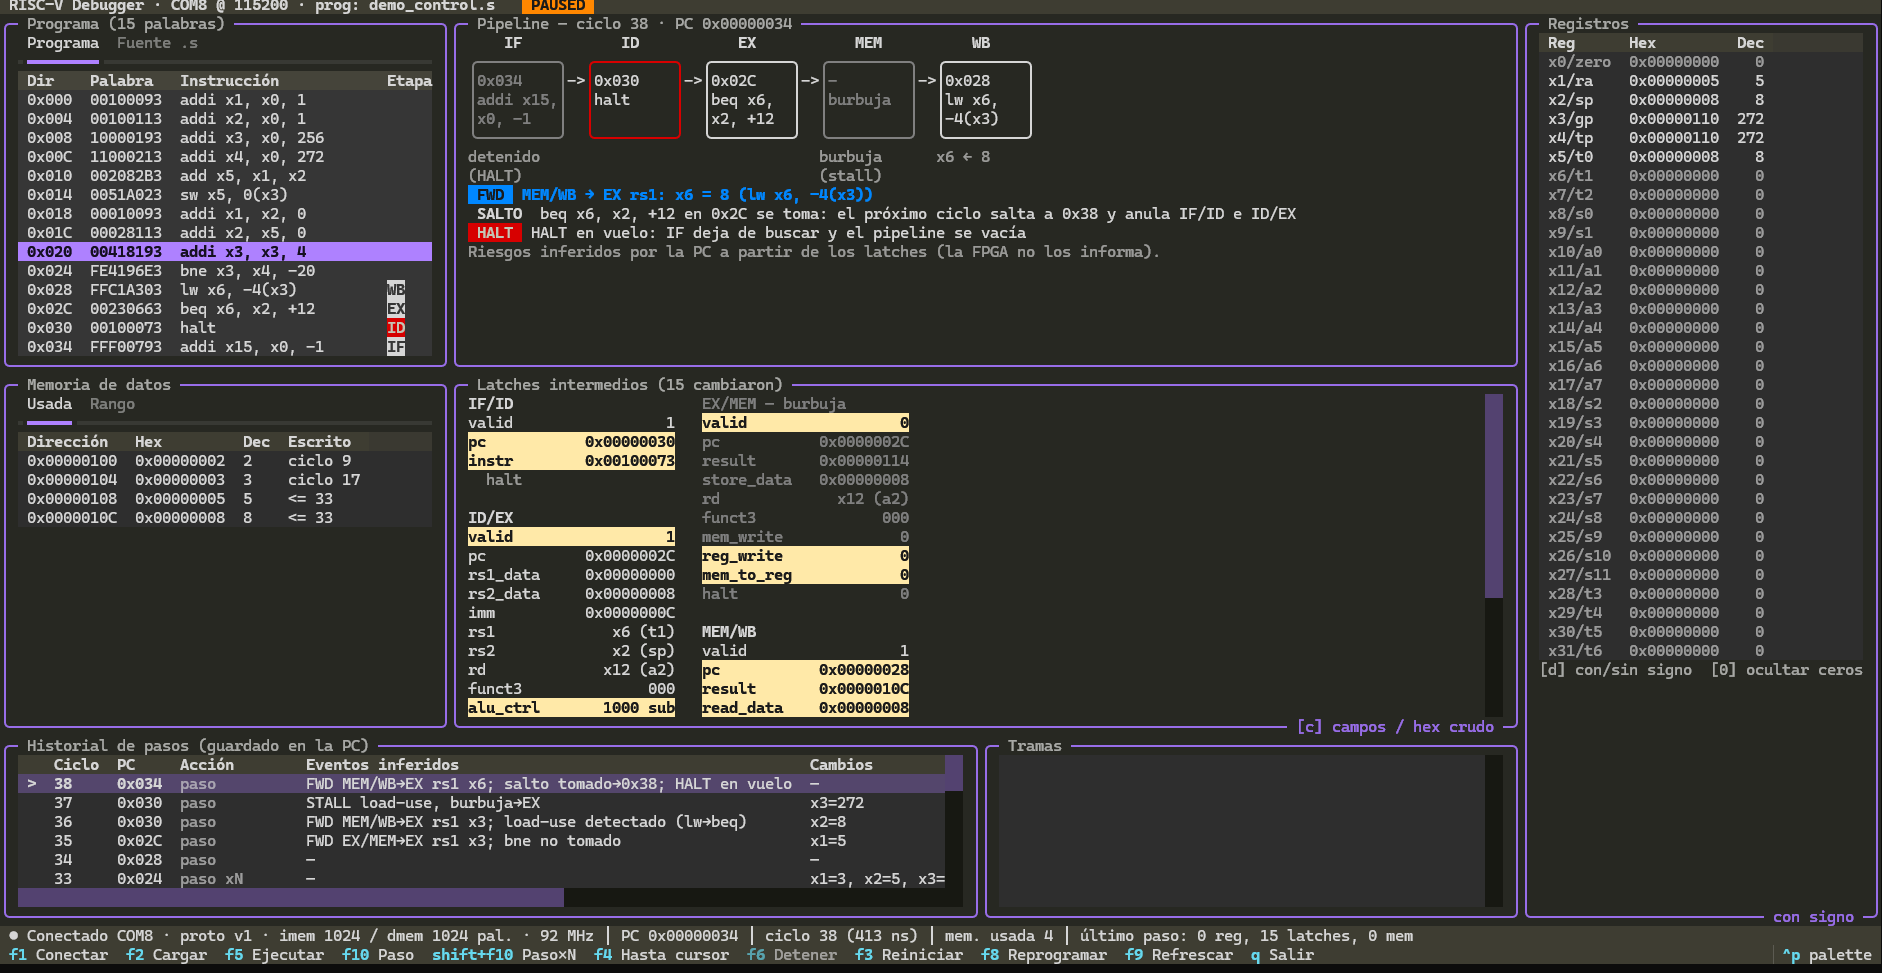
\includegraphics[width=\linewidth]{debugger_demo_control_ciclo38.png}
    \caption{Ciclo 38: el \texttt{beq} recibe \texttt{x6} desde MEM/WB y se toma; el HALT del
    camino equivocado está en ID.}
  \end{subfigure}\hfill
  \begin{subfigure}{0.49\linewidth}
    \centering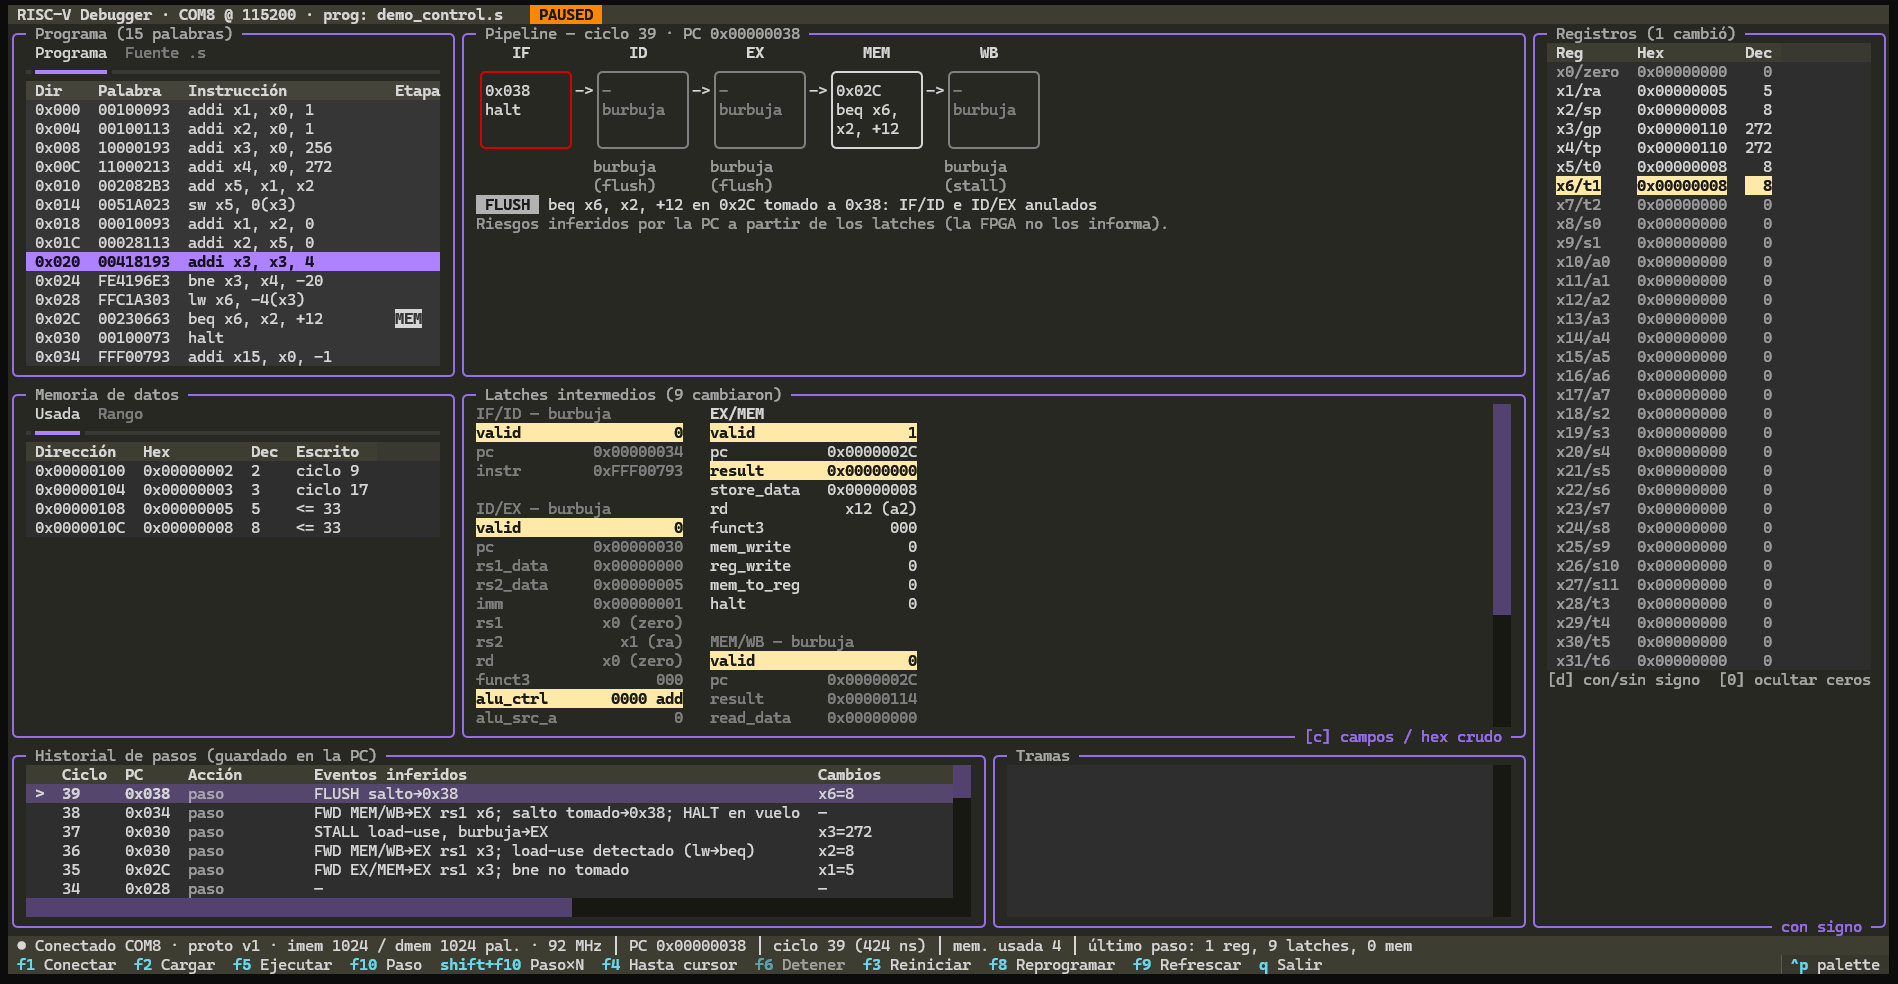
\includegraphics[width=\linewidth]{debugger_demo_control_ciclo39.png}
    \caption{Ciclo 39: flush de IF/ID e ID/EX; el HALT se anula y el core sigue en
    \texttt{PAUSED}.}
  \end{subfigure}
  \caption{\textbf{\repo{demo_control} en la placa.} El HALT en el camino equivocado no detiene el
  procesador.}
  \label{fig:demo_control}
\end{figure}

El guion de la demostración y la cobertura ciclo por ciclo están en \repo{sw/demo/README.md}.
